\documentclass[11pts]{article}
\usepackage[11pt]{moresize}
\usepackage{amsmath}
\usepackage{mathtools}
\usepackage{nccmath}
\usepackage{graphicx}
\begin{document}
	
	

{\Large Q 109: Find the vector equation of the line passing through the point 	
$\begin{psmallmatrix}1 \\2 \\-4	\end{psmallmatrix}$
and perpendicular to the two lines

$\frac{x-8}{3} = \frac{y+19}{-16}= \frac{z-10}{7} $ and\\\\
$\frac{x-15}{3} = \frac{y-29}{8}= \frac{z-5}{5} $\\

Sol:

Equation of a $\vec{l}$ passing through $\vec{a}$ and parallel to  $\vec{n}$ is given by:\\
$\vec{l} =\vec{a} + L*\vec{n} $, where L is some constant

Since the line passes through $\begin{psmallmatrix}	1 \\2 \\-4\end{psmallmatrix} \\
\vec{a} = (i + 2j - 4k)$

Let $\vec{n}$ be the normal vector to both lines. If $\vec{m}_1$ and $\vec{m}_2$ are the direction vectors of the lines,then

$\vec{m}_1^T\vec{n} = 0$

$\vec{m}_2^T\vec{n} = 0$

Let $\vec{n} = \begin{pmatrix} x \\ y \\ z\end{pmatrix} $
$\vec{m_1} = \begin{pmatrix} 3 \\ -16 \\ 7\end{pmatrix} $
$\vec{m_1} = \begin{pmatrix} 3 \\ 8 \\ -5\end{pmatrix} $\\\\
Since  $\vec{n}$ is perpendicular to $\vec{m_1}$ and $\vec{m_2}$ \\
$3x -16y + 7z = 0$\\ 
$3x + 8y - 5z = 0$\\

Solving the equations
$\frac{x}{2} = \frac{y}{3}= \frac{z}{6} = K$\\
$ x = 2K , y = 3K , z =6K$

$\vec{n} =K* (2i + 3j + 6k)$

so the equation of  $\vec{l}$ is\\
$\vec{l}=(i + 2j - 4k) + L*K (2i + 3j + 6k)$ ,where L is any constant\\

\begin{figure*}[hb]
	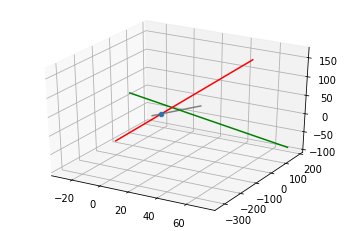
\includegraphics[width=\linewidth]{assignment1.png}
	\caption{perpendicular}
	\label{fig:1}
\end{figure*}
\end{document}